\chapter{Elekrizitätslehre}
zuerst Elektrostatik!

\section{Elektrostatik}
\subsection{Das Elektrische Feld}
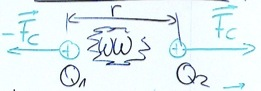
\includegraphics{Bild147} \\
\[
	F_C = \frac{1}{4 \pi \epsilon_0} \frac{Q_1 Q_2}{r^2} \\
	\epsilon_0 = \SI{8.85E-12}{\ampere\second\per\volt\metre}
\]
\uline{hier:} \\
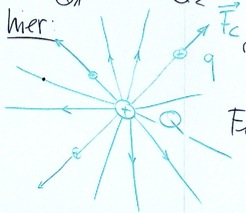
\includegraphics{Bild148}
\begin{def*}[ note = elektrische Feld , index = elektrische Feld , indexformat = {1!~2 2!1~} ]
	\[ \boxed{ \vec{E} = \frac{\vec{F_C}}{q} } \]
\end{def*}
\uline{hier:}
\[ E = \frac{1}{4 \pi \epsilon_0} \frac{Q}{r^2} \]
für Punktladung

\subsubsection{Feldlinien}
\begin{itemize}
	\item $\vec{E}$ tangential zu FL \\
		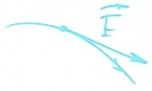
\includegraphics{Bild149}
	\item Richtungssinn!
	\item Dichte der FL $\sim \abs{\vec{E}(\vec{r})}$
	\item Vorzeichen: \\
		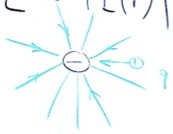
\includegraphics{Bild150}
\end{itemize}

\subsubsection{Mehrere Punktladungen}
\begin{bsp*}
	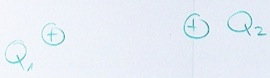
\includegraphics{Bild151} \\
	\uline{Vektoraddition!} \\
	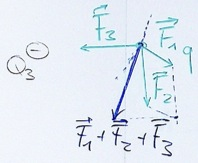
\includegraphics{Bild152}
\end{bsp*}

\subsubsection{Das Dipolfeld}
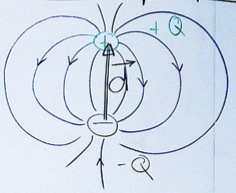
\includegraphics{Bild153}
\begin{def*}[ note = Dipolmoment , index = Dipolmoment ]
	\[ \boxed{ \vec{p} = Q \cdot \vec{d} } \]
	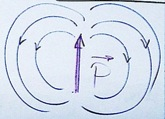
\includegraphics{Bild154}
\end{def*}

\subsubsection{Dipol in äusserem Feld}
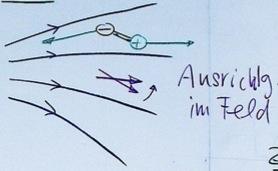
\includegraphics{Bild155} \\
\begin{itemize}
	\item Drehmoment
	\item Kraft (inhomogenes Feld)
\end{itemize}
\begin{bsp*}[ head = z.B. , note = \ce{H2O}-Molekül ]
	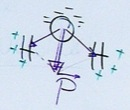
\includegraphics{Bild156}
\end{bsp*}

\subsubsection{Homogenes \texorpdfstring{$\vec{E}$}{E}-Feld}
\subsubsection{Plattenkondensator}
(kontinuierliche Ladungsverteilung) \\
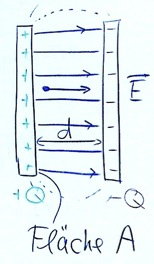
\includegraphics{Bild157} \\
Im Innern:
\[ \boxed{ E = \frac{Q}{\epsilon_0 A} } \]
Aussen: $E \approx 0$

\subsection{Die Elektrische Spannung}
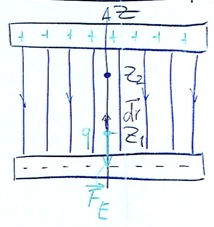
\includegraphics{Bild158} \\
Arbeit von \uline{mir}
\[
	W_{1 \rightarrow 2} = \int_{z_1}^{z_2} \vec{F} \cdot \vec{\dd r} = q E ( z_2 - z_1 ) > 0 \\
	( \vec{F} = - \vec{\overline{F_E}} = - q \vec{E} = \text{ konst. } )
\]
\begin{def*}[ note = elektrische Spannung , index = elektrische Spannung , indexformat = {1!~2 2!1~} ]
	\[
		\boxed{ U_{21} = \frac{W_{1 \rightarrow 2}}{q} }
		\intertext{( = Arbeit / Ladung )}
		[ U ] = \si{\joule\per\coulomb} = \si{\volt}
	\]
\end{def*}

\begin{rep*}[ note = Die elektrische Spannung ]
	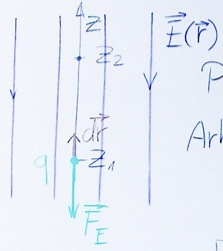
\includegraphics{Bild159} \\
	\[
		\vec{E}(\vec{r}) \text{ hier homogen} \\
		\text{Probeladung } q \\
		\text{Arbeit } W_{1 \rightarrow 2} = \int_{z_1}^{z_2} \underbrace{\vec{F}}_{\text{\enquote{meine Kraft} } \vec{F} = - \vec{F_E} = - q \cdot E} \cdot \vec{\dd r} = q \cdot E ( z_2 - z_1 )
	\]
	\begin{def*}[ note = Spannung , index = Spannung ]
		\[ U_{21} = \frac{W_{1 \rightarrow 2}}{q} \]
	\end{def*}
\end{rep*}

konservatives Kraftfeld
\begin{itemize}[ label = $\implies$ ]
	\item $W_{1 \rightarrow 2}$ unabhängig vom Weg
	\item $W_{1 \rightarrow 2} = E_{\text{pot}}(z_2) - E_{\text{pot}}(z_1)$
\end{itemize}
Das \textbf{elektrische Potential}
\[ \boxed{ \phi(x) = \frac{E_{\text{pot}}(z)}{q} } \]
$\implies U_{21} = \phi(z_2) - \phi(z_1)$ \\
Spannung = Potenitaldifferenz
\begin{bsp*}
	hier $W_{1 \rightarrow 2} > 0$ \\
	$z_2$ liegt auf höherem Potential
\end{bsp*}

\subsection{Bewegung \texorpdfstring{$\perp$}{senkrecht zum} \texorpdfstring{$\vec{E}$}{E}-Feld}
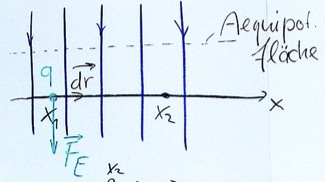
\includegraphics{Bild160}
\[ \begin{split}
	W_{1 \rightarrow 2}
		&= \int_{x_1}^{x_2} \vec{F} \cdot \vec{\dd r} = 0 \\
		&= U_{21} = 0 \\
		&= \phi(x_2) - \phi(x_1)
\end{split} \]
\begin{bsp*}[ note = Plattenkondensator ]
	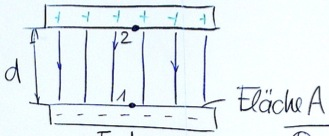
\includegraphics{Bild161}
	\[ U_{21} = - \frac{qEd}{q} = \underbrace{Ed}_{E = \frac{Q}{\epsilon_0 A}} = \frac{Qd}{\epsilon_0 A} \]
	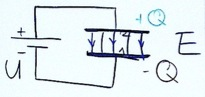
\includegraphics{Bild162}
	\[ U_{21} = U \implies E = \frac{U}{d} \quad \left[ \si{\volt\per\metre} \right] \]
\end{bsp*}
\begin{def*}[ note = Kapazität , index = Kapazität ]
	\[ C = \frac{Q}{U} \]
	
	\[ \text{Plattenkondensator } C = \frac{\epsilon_0 A}{d} \]
\end{def*}

\subsubsection{Beliebiges \texorpdfstring{$\vec{E}$}{E}-Feld}
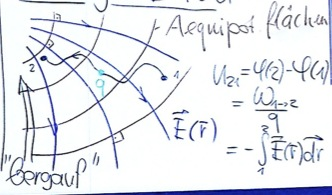
\includegraphics{Bild163}
\[ \begin{split}
	U_{21}
		&= \phi(2) - \phi(1) \\
		&= \frac{W_{1 \rightarrow 2}}{q} \\
		&= - \int_{1}^{2} \vec{E}(\vec{r}) \vec{\dd r}
\end{split} \]

\subsubsection{Beschleunigung in Röntgenröhre}
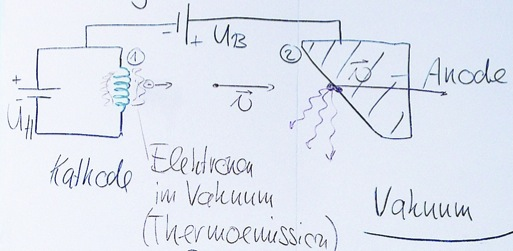
\includegraphics{Bild164}
\[
	\left. \begin{matrix*}[l]
		\phi(2) > \phi(1) \\
		q = -e
	\end{matrix*} \right\} \quad E_{\text{pot}}(2) < E_{\text{pot}}(1) \\
	\text{EEH: } -e \phi(1) + \underbrace{\frac{1}{2} m v_1^2}_{0} = -e \phi(2) + \frac{1}{2} m v_2^2 \\
	\implies \frac{1}{2} m v_2^2 = e ( \phi(2) - \phi(1) ) = e \cdot U_B
\]

\subsubsection{Materialien in elektrischen Feldern}
\subsubsection{Metalle}
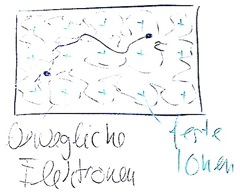
\includegraphics{Bild165} \\
laden \\
\begin{tabular}{ l l }
	$+Q$ &Elektronen weg \\
	$-Q$ &Elektronen dazu
\end{tabular}

\subsubsection{Isolator}
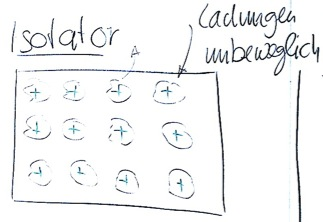
\includegraphics{Bild166}

\subsubsection{Metalle}
Elektrostatik $\vec{v} = \vec{0}$
\begin{itemize}[ label = $\implies$ ]
	\item im Innern $\vec{E} = \vec{0}$
	\item Metalle sind Aequipotentialgebiete
\end{itemize}
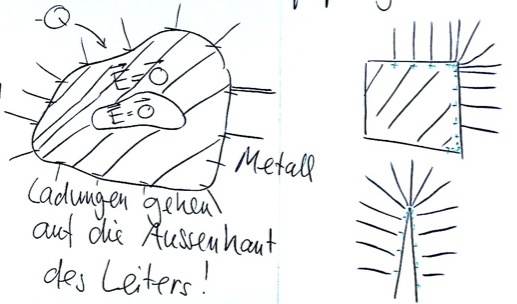
\includegraphics{Bild167}

\subsubsection{Metall in äusserem Feld}
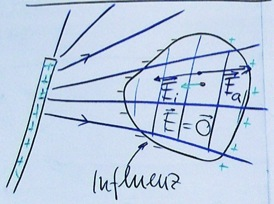
\includegraphics{Bild168} \\
Elektrometer \\
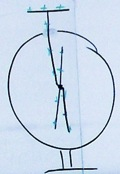
\includegraphics{Bild169}

\subsubsection{Isolator im äusseren Feld}
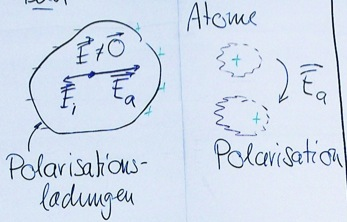
\includegraphics{Bild170}

\subsection{Elektrische Gleichströme: Leiter}
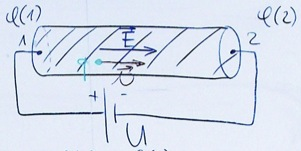
\includegraphics{Bild171} \\
\begin{itemize}[ label = $\implies$ ]
	\item $\phi(1) > \phi(2)$
	\item keine Aequipotentialfläche
\end{itemize}
$\vec{E}$-Feld beschleunigt Ladungen \\
Reibung an Ionen bremst sie \\
$\implies \vec{v} =$ konst.

\begin{rep*}[ note = Elekrische Spannung - elektrisches Potential ]
	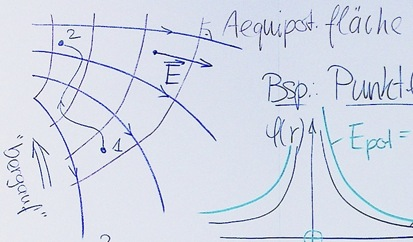
\includegraphics{Bild172}
	\[ U_{21} = - \int_1^2 \vec{E} \cdot \vec{\dd r} \]
	\begin{bsp*}[ note = Punktladung ]
		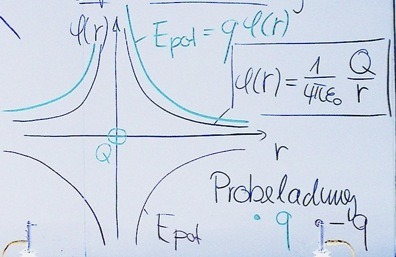
\includegraphics{Bild173}
	\end{bsp*}
\end{rep*}

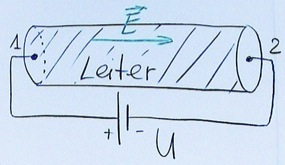
\includegraphics{Bild174}
\[ U_{21} = U \]
\begin{itemize}[ label = $\implies$ ]
	\item $\vec{E} \neq \vec{0}$ im Leiter
	\item Ladungsträger beschleunigt
\end{itemize}
+ Reibung $\implies$ $\vec{v} = $ konst. \\
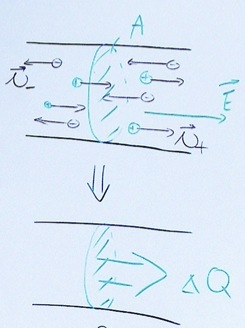
\includegraphics{Bild175} \\
pos. Stromrichtung in Feldrichtung
\begin{def*}[ note = Stromstärke , index = Stromstärke ]
	\[ \boxed{ I = \frac{\increment Q}{\increment t} } \quad [ \si{\ampere} ] \]
\end{def*}
\begin{def*}[ note = Stromdichte , index = Stromdichte ]
	\[
		\boxed{ \vec{j} = \rho \cdot \vec{v} } \quad \left[ \si{\ampere\per\metre\squared} \right] \\
		\text{mit Ladungsdichte } \rho = \underbrace*{n}_{\text{Teilchendichte}} \cdot \underbrace*{z}_{\text{Ladung pro Teilchen}} \cdot \underbrace*{e}_{\text{Elementarladung } \approx \SI{1.6E-19}{\coulomb}}
	\]
\end{def*}

\subsubsection{Metalle}
i.A. Elektronen: $z = -1$

\subsubsection{Elektrolyt}
\[ \vec{j} = \vec{j_{+}} + \vec{j_{-}} = n_{+} z_{+} e \vec{v_{+}} + n_{-} z_{-} e \vec{v_{-}} \]
\begin{bsp*}[ head = z.B. ]
	\ce{Mg2+}-Ionen: $z = +2$
\end{bsp*}

In zylindrischem Leiter: \\
homogene Stromdichte \\
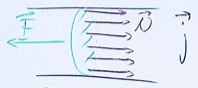
\includegraphics{Bild176}
\[ I = A j \implies j = \frac{I}{A} \]

\subsubsection{Inhomogenes \texorpdfstring{$\vec{j}(\vec{r})$}{j(r)}}
\begin{bsp*}[ note = Elektrolyt ]
	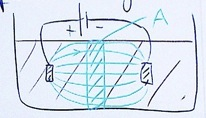
\includegraphics{Bild177}
	\[ I = \iint_A \vec{j} \cdot \vec{\dd A} \]
\end{bsp*}

\subsection{Strömungsgesetze}
\[ \begin{matrix*}[l]
	\text{\uline{Hyrdo:} } & I_V = \frac{p_1 - p_2}{\underbrace{R_V}_{\text{innere}\\\text{Reibung}}} \\
	\text{\uline{el. Strom:} } & I = \frac{U}{\underbrace{R}_{\text{Reibung}\\\text{an Ionen,}\\\text{Elektronen}}}
\end{matrix*} \implies \]
\begin{def*}[ note = elekrischer Widerstand , index = elektrischer Widerstand , indexformat = {12 2!1~} ]
	\[ \boxed{ R = \frac{U}{I} } \quad [ \si{\ohm} ] \]
	hängt ab von
	\begin{itemize}
		\item Material ($\rightarrow$ spez. Widerstand $\rho_W$)
		\item Form \\
			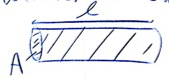
\includegraphics{Bild178}
			\[ R = \rho_W \frac{l}{A} \]
	\end{itemize}
\end{def*}

\subsection{Strom-Spannung-Charakteristik}
\subsubsection{Metall}
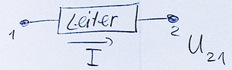
\includegraphics{Bild179} \\
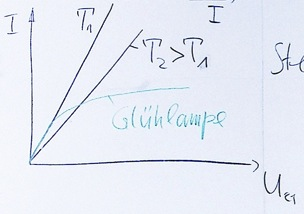
\includegraphics{Bild180} \\
Steigung: $\frac{I}{U}$ \\
$\implies R = \frac{U}{I} = $ konst. \\
Ohmsches Gesetz

\subsection{Joulsche Wärme}
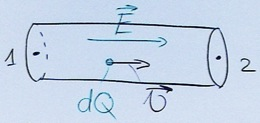
\includegraphics{Bild181} \\
$\vec{E}$-Feld leistet Arbeit (Batterie!)
\[ \dd W_{1 \rightarrow 2} = \dd Q \cdot U_{21} \]
$\implies$ \uline{elektrische Leistung}:
\[
	\boxed{ P = U \cdot I } \\
	P = \frac{\dd W_{1 \rightarrow 2}}{\dd t} = \underbrace{\frac{\dd Q}{\dd t}}_{I} \cdot U_{21} \\
	[ W ] = \si{\volt\ampere}
\]

\subsection{Elektrische Leitfähigkeit}
\[ I = \frac{1}{R} \cdot U \rightarrow \boxed{ \vec{j} = \sigma \cdot \vec{E} } \quad (\text{von } \vec{j} = \rho \cdot \vec{v}) \]
Bilanzgewinnung im ganzen Leiter \\
vektorielles Gesetz gilt überall im Leiter \\
\begin{def*}[note = elektrische Leitfähigkeit , index = elektrische Leitfähigkeit , indexformat = {12 2!1~} ]
	\[ \sigma = \frac{1}{\underbrace{\rho_W}_{\text{spez. Widerstand}}} \]
\end{def*}

\subsection{Elektrokardiogramm}
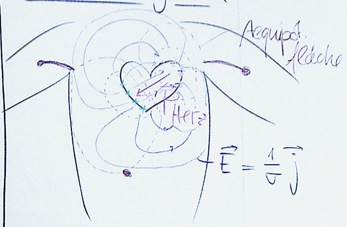
\includegraphics{Bild182}

\subsection{Spannungsquellen}
\begin{bsp*}[ note = Batterie ]
	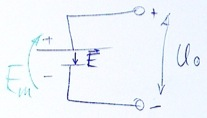
\includegraphics{Bild183}
\end{bsp*}
\enquote{Elektromotorische Kraft} (EMK)
\[ E_m = \frac{W_{1 \rightarrow 2}}{q} \]
Leerlaufspannung $U_0 = E_m$
\begin{bsp*}[ note = Das Ruhepotential einer Zelle ]
	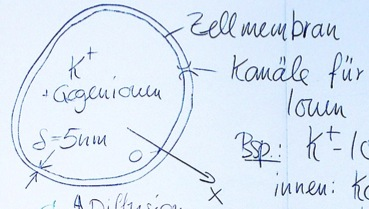
\includegraphics{Bild184} \\
	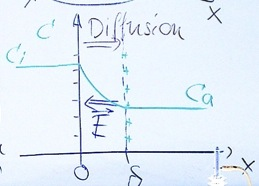
\includegraphics{Bild185}
	\begin{bsp*}
		\ce{K+}-Ionen \\
		innen Konz. $c_i$ \\
		aussen Konz. $c_a$ \\
		Im GGW sorgt Körper für $c_i > c_a$
		
		\uline{Lösung:} Konzentration in der Zellwand
		\[
			c(x) = c_i e^{-\frac{z e \cdot E \cdot x}{kT} }
			\intertext{am äusseren Rand}
			c(\delta) = c_a = c_i e^{-\frac{z e \cdot \overbrace{E \cdot \delta}^{\text{Diff. Spannung}}}{kT}}
			\intertext{Diff'spannung $U_D= E \delta$}
			\boxed{ U_D = \frac{kT}{z \cdot e} \ln \frac{c_i}{c_a} }
		\]
		Ruhepotential $U_D \approx \SI{90}{\milli\electronvolt}$
	\end{bsp*}
\end{bsp*}

\begin{rep*}[ note = El. Gleichströme ]
	\[
		\begin{matrix*}[l]
			\text{\uline{Stromstärke:} } &\boxed{ I = \frac{\increment Q}{\increment t} } \\
			\text{\uline{Stromdichte:} } &\boxed{ \vec{j} = \rho \cdot \vec{v} }
		\end{matrix*}
		\intertext{Strömungsgesetze:}
		\boxed{ I = \frac{U}{R} } \quad \boxed{ \vec{j} = \sigma \cdot \vec{E} }
	\]
	
	\uline{Spannungsquellen}
	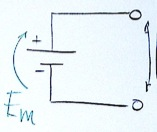
\includegraphics{Bild186} \\
	$E_m$: elektromotorische \enquote{Kraft} \\
	$\implies$ Arbeit, um Ladung gegen E-Feld zu verschieben
	\begin{bsp*}[ note = Zellmembran ]
		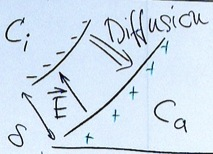
\includegraphics{Bild187} \\
		$c_i > c_a$ \\
		\ce{K+}-Konzentration \\
		$\delta = \SI{5}{\milli\metre}$ \\
		Diffusion transportiert Ladungen (\ce{K+}) gegen E-Feld
		\[
			\implies U_D = \frac{kT}{ze} \ln \frac{c_i}{c_a} \\
			\text{Ruhepotential } \approx \SI{90}{\milli\volt} \\
			E = \frac{U_D}{\delta} = \frac{\SI{90E-3}{\volt}}{\SI{5E-9}{\metre}} = \SI{2E7}{\volt\per\metre}
		\]
	\end{bsp*}
\end{rep*}

\subsubsection{Reale Spannungsquellen}
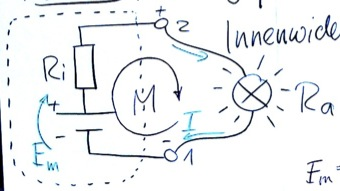
\includegraphics{Bild188} \\
Innenwiderstand $R_i$
Spannungsabfall am $R_i$
\[ U_i = I \cdot R_i \]
Klemmanspannung
\[ U_{21} = E_m - I \cdot R_i = U_0 - I \cdot R_i \]
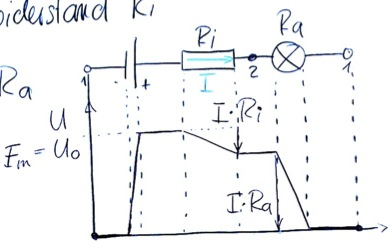
\includegraphics{Bild189} \\
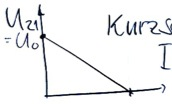
\includegraphics{Bild190} \\
Kurzschluss:
\[ I_{\text{max}} = \frac{U_0}{R_i} \]

\subsection{Kirchhoffsche Maschenregel}
\[ \boxed{ \sum E_m = \underbrace{\sum U_i}_{\text{alle Spannungsabfälle}} } \]

\subsubsection{Kirchoffsche Knotenregel}
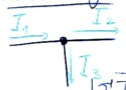
\includegraphics{Bild191} \\
Hier $I_1 = I_2 + I_3$
\[ \boxed{ \sum I_{\text{zufl.}} = \sum I_{\text{abfl.}} } \]
(Kontinuitätsgleichung)

\uline{Wichtig: Vorzeichen}
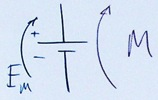
\includegraphics{Bild192} $E_M$ positiv \\
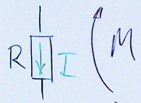
\includegraphics{Bild193} $I \cdot R$ negativ \\
\uline{Rezept:}
\begin{enumerate}[ label = \arabic*) ]
	\item Stromrichtungen einzeichnen (beliebig)
	\item Knotenregel anwenden
	\item Maschenregel anwenden
	\item Gleichungen nach $I_1 , I_2, \dots$ auflösen
\end{enumerate}
